\chapter{Results}\label{chap:Results}
In this chapter, I will present the evaluations an evaluation of the implementation and optimizations described in this thesis, which will be refered to here as UHCAF.

\section{Experiment Setup}
\textbf{Stampede} is a supercomputer at the Texas Advanced Computing Center
(TACC). It uses Dell PowerEdge server nodes, each with two Intel Xeon E5 Sandy
Bridge processors (16 total cores) and 32 GiB of main memory per node. Each
node also contains a Xeon Phi coprocessor, but we did not use this in our
experimentation. The PowerEdge nodes are connected through a Mellanox FDR
InfiniBand network, arranged in a 2-level fat tree topology. 
%Stampede includes MPICH2 and MVAPICH2-X. 
We installed OpenUH 3.0.40, Rice CAF 2.0 (r4169), GASNet 1.22.4, and the
latest GASNet 1.24.2 on Stampede for evaluations. The MPI implementation we used was MVAPICH2, version 1.9a2.

\section{Benchmarks}
\subsection{Team Microbenchmark}
\subsubsection{Evaluation of Form\_Team}
\begin{figure}[h]
  \centering
  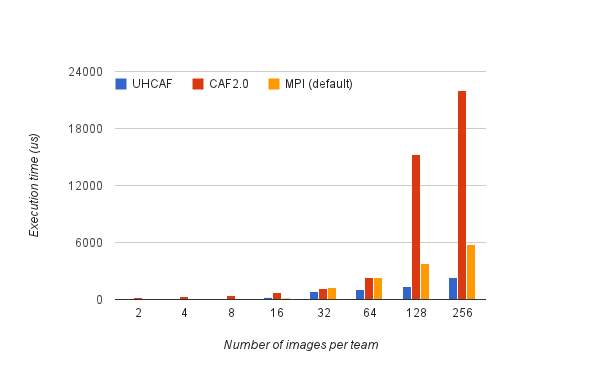
\includegraphics[width=\columnwidth]{figures/form-team.png}
  \caption{Comparison of FORM\_TEAM}
  \label{fig:form-team}
\end{figure}
\subsubsection{Evaluation of Team Barriers}
%Edit by Gracia
In Figure~\ref{fig:stampede-team-barrier}, we show timings for different use
cases of team barriers. We arranged 4096 images to show 3 synchronization cases: 1)
all participating images synchronize using \texttt{sync all}, 2) form
teams and have images in each team synchronize using \texttt{sync team}, and
3) image subsets synchronize using \texttt{sync images}.  Logically, the
\texttt{sync images} statement with an image list consisting of all images in
the same logical ``team'' will have the same effect as
a \texttt{sync team} statement using a team variable representing a team
consisting of the same images.

\begin{figure}[h]
  \centering
  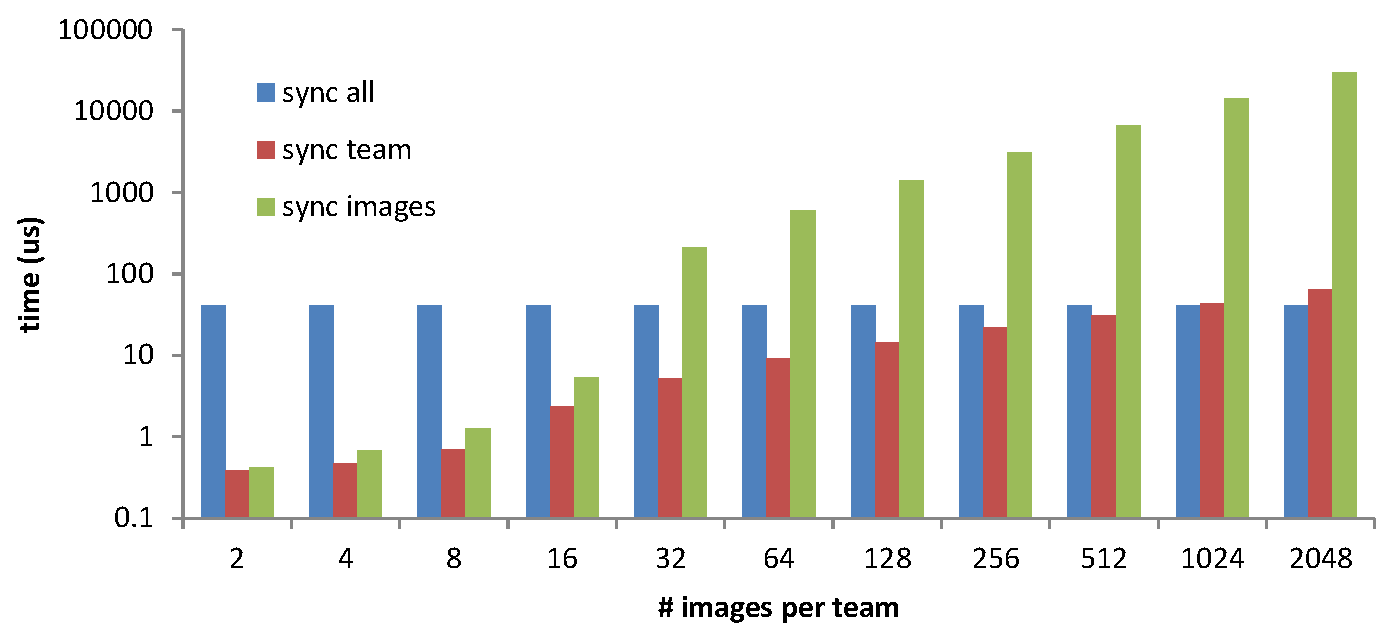
\includegraphics[width=\columnwidth]{figures/stampede-team-barrier-4096.eps}
  \caption{Barrier synchronization for groups of images (4096 total images), on Stampede.}
  \label{fig:stampede-team-barrier}
\end{figure}

The reader may notice that having all participating images execute
\texttt{sync all} performs reasonably well until the number of images per team
reduces past a certain threshold. This is because we utilized the barrier
provided by GASNet to implement \texttt{sync all} for the initial team, and it
happens to be well tuned for the InfiniBand interconnect used on Stampede.
Before \texttt{sync~team} was proposed, synchronization among a subset of
images could be achieved alternatively using the \texttt{sync~images}
statement.  The scalability for this statement, however, quickly became an
issue as the participating images increase, since the semantics of this
statement require that an image perform a point-to-point synchronization with
each image in its specified image list.  We observe here that \texttt{sync team} is
a far more effective approach for synchronizing a subset of images compared to
using \texttt{sync images}.

\begin{figure}[h]
    \centering
    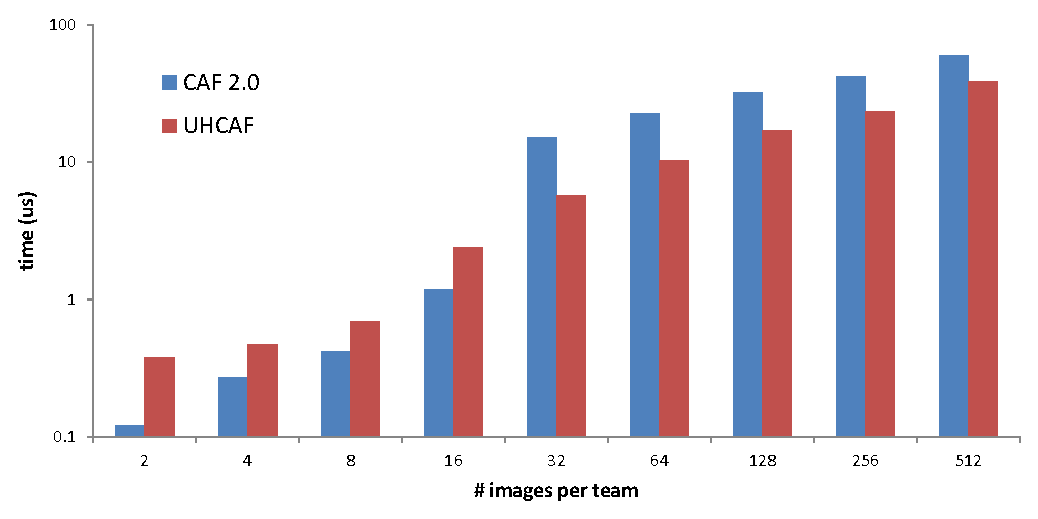
\includegraphics[width=\columnwidth]{figures/team-barrier-stampede-1024.eps}
    \caption{Comparison of team barrier between UHCAF and CAF 2.0 (1024 total
    images), on Stampede.}
    \label{fig:stampede-teambar-caf2}
\end{figure}

We also compared the performance of our team barrier implementation with the
equivalent \texttt{team\_barrier()} routine available in the Rice CAF 2.0
implementation, shown in Figure~\ref{fig:stampede-teambar-caf2}.  For this
comparison, we used the most recent GASNet version, 1.24.2 (all other
experiments described in this section used GASnet 1.22.4).  The result shows
that the CAF 2.0 barrier implementation was more efficient when the team size
was less than or equal to 16, where all images in a team reside within the
same compute node. On the other hand, our barrier implementation was more
efficient when each team spans multiple compute nodes.  We attribute this
result to the 2-level barrier algorithm we've implemented, while there is
evidently some improvements to be made in our intra-node barrier
implementation.

\subsection{Reduction}

In the two charts in Figure~\ref{fig:reduction}, we compare the application of
our  2-level optimization on the reduction operation to the original implementation,
which uses the recursive doubling algorithm~\cite{doubling}. The two-level implementation uses binomial tree reduction from non-leaders to their node leader; then, a recursive-doubling all-reduce is performed between the leaders; and finally the non-leaders perform parallel local gets from their leader. We also compare it to CAF 2.0, Open MPI and MVAPICH. As expected, the memory hierarchy awareness in our two-level algorithm gives very good results (note the case where we have 8 images
per node). 
\begin{figure*}[!h]
\begin{minipage}[!h]{\linewidth}
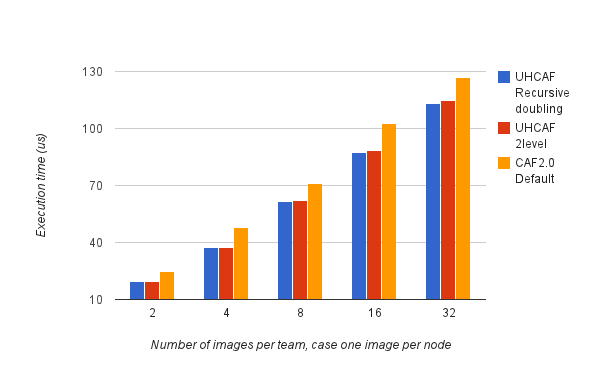
\includegraphics[width=3.5in, height=2in]{figures/reduction-1ipn-team.png}
%\caption{Performance evaluations for TDLB  barrier algorithm within teams using the Teams Microbenchmarks} 
%\includegraphics[width=2.4in, height=1.8in]{figure/is_A.eps}
\end{minipage}
\quad
\begin{minipage}[!h]{\linewidth}
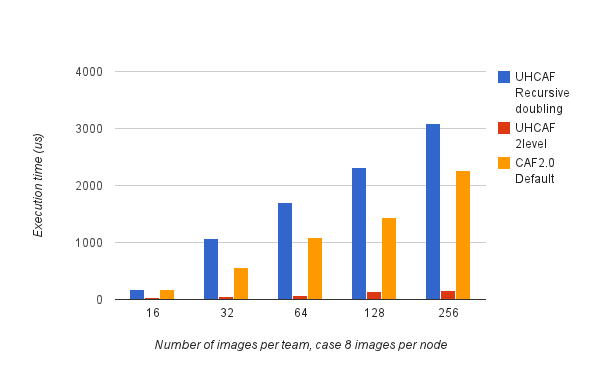
\includegraphics[width=3.5in, height=2in]{figures/reduction-8ipn-team.png}
%\caption{Performance evaluations for TDLB  barrier algorithm within teams using the Teams Microbenchmarks} 
%\includegraphics[width=2.4in, height=1.8in]{figure/is_A.eps}
\end{minipage}
\caption{Performance evaluations for the 2-level reduction algorithm using the Teams Microbenchmark suite} 
\label{fig:reduction}
\end{figure*}


In the case of one image per node, not only is there no additional overhead compared to
the original implementation, but we were able to improve the performance by
applying a further optimization. Using the 2-level approach advocated in this thesis, we can
distinguish remote memory operations that access out-of-node memory via the
interconnect's RDMA from memory accesses within the node. In the former case,
we can employ the canary protocol~\cite{canary}, which entails the target
polling on the last byte (or some bytes) as a canary value to check for
communication completion (a valid approach because an RDMA write over
Infiniband can be assumed to complete in byte order). By using this protocol,
which effectively bundles a notification of completion with the data to be
sent, we can eliminate sending an additional notification per write in our
implementation.\\

\subsection{Using Team-based Collectives for CG}
\begin{figure}[h]
\centering
%\includegraphics[width=\columnwidth]{figures/nas-cg-whale-teams.png}
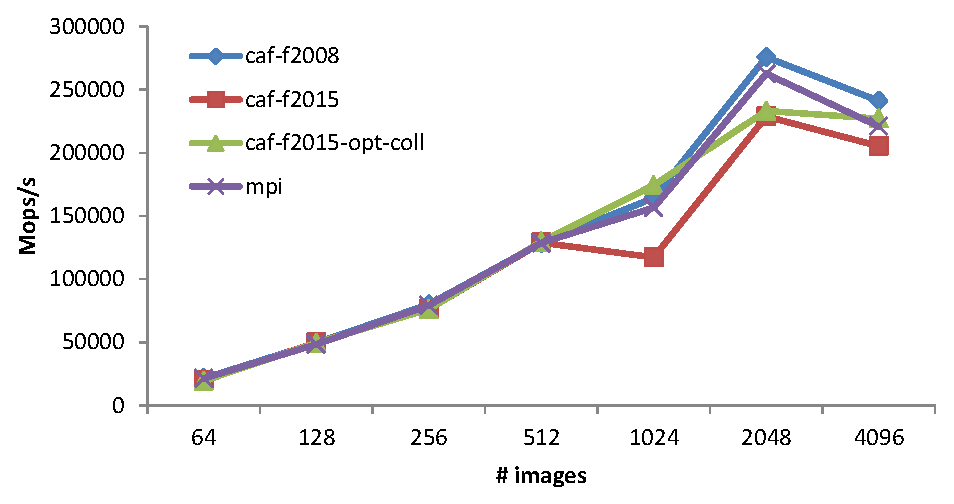
\includegraphics[width=\columnwidth]{figures/stampede-caf-cg-D.eps}
\caption{CG benchmark (class D) on Stampede, using 16 images per node}
\label{fig:cg-stampede}
\end{figure}

To assess the potential benefits of using the teams and collectives features,
we updated our CAF implementation of the CG benchmark from the NAS Parallel
Benchmarks (NPB) suite (available in \cite{caf-testsuite}).
The CG benchmark uses the \textit{conjugate gradient} method to approximate
the eigenvalue of a sparse, symmetric positive definite matrix, and makes use
of unstructured matrix vector multiplication. We first ported this benchmark
to use Fortran coarrays, adhering to the Fortran 2008 specification. For the
extended version, we grouped the images into \textit{row teams}, and during
the execution of the conjugate gradient method we performed the sum reductions
with respect to these teams. In this way, we were able to assess the utility
of both the teams and reduction features that are expected to be included in
Fortran 2015.

In Figure~\ref{fig:cg-stampede}, we compare the results achieved with this new
implementation on Stampede using class D problem size with our original Fortran 2008 version of the
benchmark. We also show the results executing the original MPI version of CG
using MVAPICH2. % and an MPI version of the benchmark using Open MPI 1.8.3.
The baseline collectives implementation resulted in regressed performance
relative to the Fortran 2008 version. Through synchronization-hiding
and locality-aware optimizations of these collective operations, as described
in Section~\ref{sec:collectives}, we were able to improve on the baseline
performance. However, we observed scalability issues even when using our
optimized reductions when running with 2048 and 4096 images. We believe the
issue originates from the need to add the \texttt{change~team} and
\texttt{end~team} statements before and after calls to \texttt{co\_sum} for
performing the row-based reductions. The \texttt{end-team} statement, in
particular, entails a barrier synchronization for all images in the initial
team. One way around this would be to surround the entire iterative loop
executed in \textit{conj\_grad} inside a team block, and utilize the new
image selection syntax (e.g., $a(j)[i, team$=$init\_team]$) to perform the
necessary communication and synchronization operations across teams (e.g. for
the transpose operation). However, we have not yet implemented this
image selection feature.

%\section{Applications}
%\subsection{Parallel Sort}
%[In progress]
%BigSort is an application implemented distributed sorting algorithm. In this applicaiton, we shows the usage and benefit of node team, the extension I proposed in this work. 


